  \subsection{Le théorème de CAP }
  \label{sec:cap}

  \acrshort{cap} \cite{brewer2000towards} est l'acronyme de
  \textit{``\textbf{C}onsistency, \textbf{A}vailability and
    \textbf{P}artition Tolerance''}, ou \textit{``Cohérence,
    Disponibilité et Résistance au partitionnement''}. Ce théorème
  explique qu'il est impossible qu'un système distribué satisfasse
  simultanément aux trois contraintes suivantes:

  \begin{itemize}
  \item [Cohérence]: tous les nœuds du système voient exactement les
    mêmes données au même moment.

  \item [Disponibilité]: la perte de nœuds n'empêche pas les survivants
    de continuer à fonctionner correctement.

  \item [Résistance au partitionnement]: aucune panne moins importante
    qu'une coupure totale du réseau ne doit empêcher le système de
    répondre correctement (ou encore : en cas de partitionnement ,
    chacune des partitions doit pouvoir fonctionner de manière
    autonome).
  \end{itemize}

  \begin{figure}[h]
    \centering
    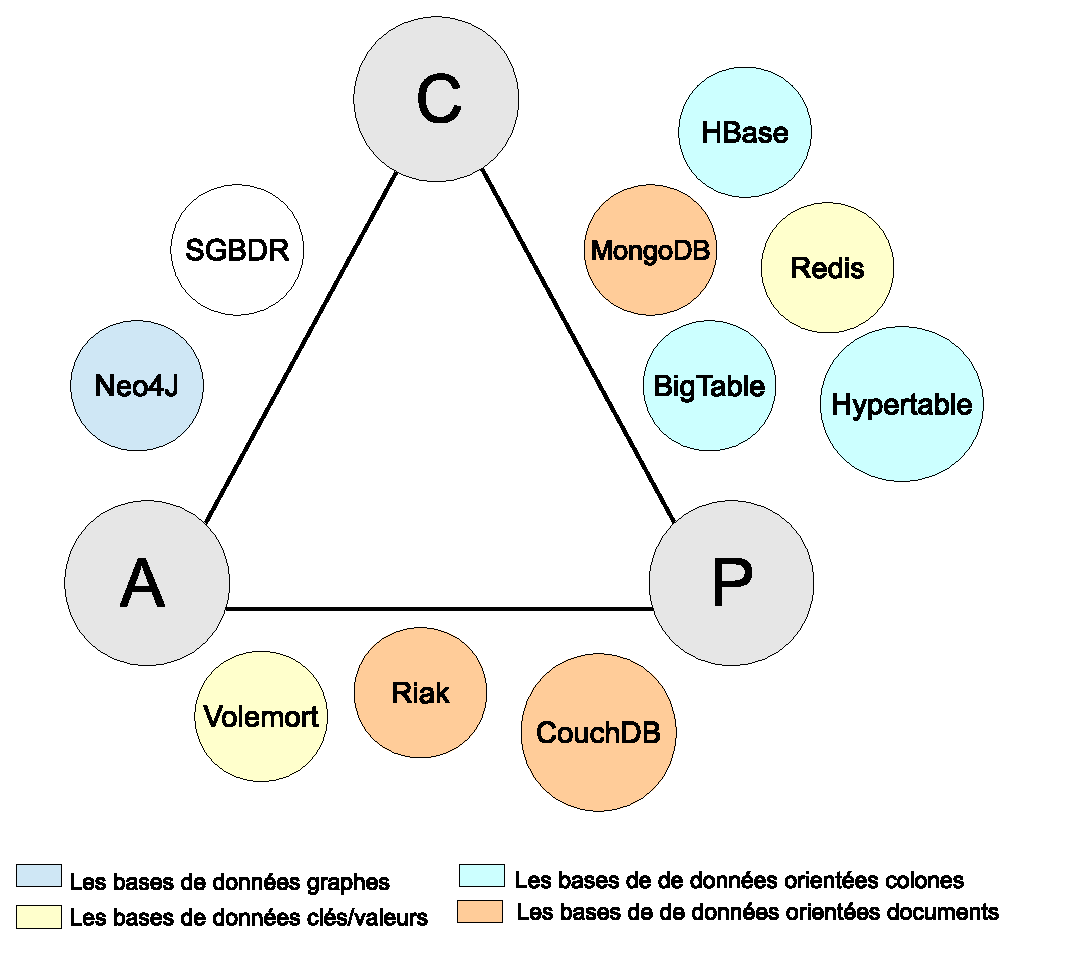
\includegraphics[width=0.96\textwidth]{figs/cap.eps}
    \caption{Le théorème CAP}
    \label{fig:cap}
\end{figure}

%%% Local Variables:
%%% mode: latex
%%% TeX-master: "../main"
%%% End:


  Le théorème de \acrshort{cap} stipule qu'il est impossible d'obtenir
  ces trois propriétés en même temps dans un système distribué et
  qu'il faut donc en choisir deux parmi les trois, Les bases de
  données relationnelles implémentent les propriétés de cohérence et
  de disponibilité (système \emph{CA}). Les bases de données
  \emph{NoSQL} sont généralement des systèmes \emph{CP} (cohérent et
  résistant au partitionnement) ou \emph{AP} (disponible et résistant
  au partitionnement), la figure \ref{fig:cap} présente le
  positionnement de quelque systèmes \emph{NoSQL} par rapport au
  théorème \acrshort{cap}.

%%% Local Variables:
%%% mode: latex
%%% TeX-master: "../main"
%%% End:
